\begin{event}{OpenDreamKit Kickoff meeting}{kickoff}{Orsay (France) 2015-09-02 to 2015-09-05}{PS,UK,LL,SA,JU,UW,USH,UV,ZH,USO,US,UJF,SR}{34}{http://opendreamkit.org/2015/09/02/KickoffMeeting/}

\textbf{Main goals.} This was the starting event of the project, allowing for everyone to meet and start working.

\textbf{ODK implication.} As a lead partner, Paris-Sud was chosen to host the event. 30 ODK participants were present, 
representing most of the partners.

\textbf{Event summary.} Part of event was dedicated to ODK-specific tasks and administrative questions. But the goal
was to make much more out of it. We planned for many technichal talks, presenting existing and emerging technologies
related to ODK. We also had two days of coding sprints to start working right away on ODK tasks.

\textbf{Demographic.} Most of the participants were from ODK but we had invited a few external participants.

\textbf{Results and impact.} This event set the tone for up-comming development workshops by creating a friendly, instructive, 
working atmosphere. It also set the different goals of project, allowing everyone to share their views and
understanding of ODK tasks.

\begin{figure}[ht]
\caption*{ODK Kickoff meeting}
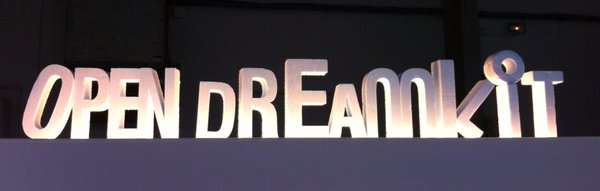
\includegraphics[scale=0.3]{pictures/kickoff1.jpg}

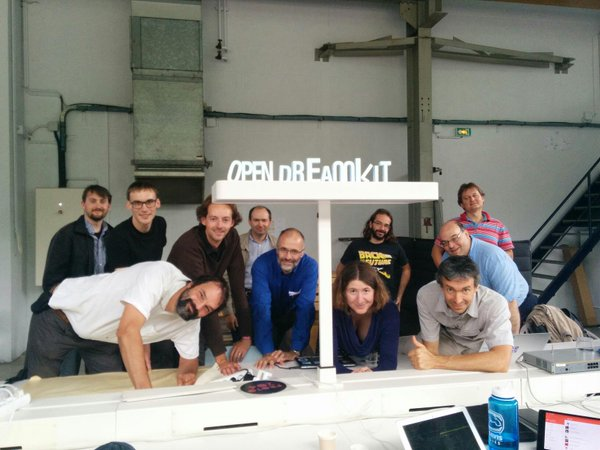
\includegraphics[scale=0.5]{pictures/kickoff2.jpg}
\end{figure}



\end{event}